\chapter{El criptosistema RSA}

\begin{defn}[Función trampa]
También conocida como función ratonera, se trata de una función $f_e$ de un sólo sentido que depende de un parámetro $e$ conocido como \textbf{clave pública}, tal que su inversa $f^{-1}_d$ depende de un parámetro $d$ conocido como \textbf{clave privada} y $d$ sólo se puede calcular a partir de $e$ con ayuda de información adicional.
\end{defn}

La idea del \textbf{RSA}, criptosistema que estudiaremos a continuación, consiste en el uso de este tipo de funciones apoyándose en la idea de que encontrar primos es \textbf{fácil} pero factorizar un número grande en primos es \textbf{difícil}

\section{Generación de claves}
Los pasos a seguir son:
\begin{enumerate}
\item Generamos dos números primos $p,q$ grandes que, como nos ha mostrado el profesor en clase, es algo fácil de realizar.

Más adelante veremos cómo se generan estos primos.

\item Encontramos un número $e$ coprimo con $(p-1)(q-1)$.

Para hacerlo empleamos el algoritmo de Euclides, empezando con un número cualquiera $e\in [1, (p-1)(q-1)]$ y le aplicamos el algoritmo de Euclides para obtener el máximo común divisor.

En caso de que este máximo común divisor no sea 1, simplemente probamos con otro número hasta dar con la clave.

\item Encontramos el número $d$ inverso de $e$

Cuando tenemos el número $e$, podremos apoyarnos en la identidad de Bezout para obtener su inverso.

\item Calculamos $n=p\cdot q$

\item Publicamos la clave pública $[n,e]$ y mantenemos oculta la clave para descifrar $d$.
\end{enumerate}

Hay un punto importante de este procedimiento que puede hacernos dudar: la búsqueda del número $e$, puesto que el algoritmo de Euclides podría llevarnos mucho tiempo.

No obstante el algoritmo de Euclides es muy rápido, cosa que podemos comprobar basándonos en el siguiente lema:
\begin{lemma}
Al aplicar el algoritmo de Euclides, siendo $r_n$ el resto obtenido en la iteración $n$, se cumple que:
\[r_{n+2} < \frac{1}{2}r_n\]
\end{lemma}
\begin{corol}
El número de pasos necesarios hasta completar el algoritmo de Euclides es $2\log(N)=O(\log(N))$.

Por tanto, el tiempo necesario para completar el algoritmo es $O(\log(N)^3)$
\end{corol}

Veamos ahora la demostración del lema:
\begin{proof}
Para empezar, observamos que si $r_{n+1} \leq \frac{1}{2}r_n$ no tenemos nada más que hacer, puesto que los restos van decreciendo siempre.

Por otro lado, si
\[r_{n+1} > \frac{1}{2} r_n \implies 2r_{n+1} > r_n\]

Pero sabemos que
\[r_n = r_{n+1} + r_{n+2} \implies r_{n+2} = r_n-r_{n+1} < r_n-\frac{1}{2}r_n = \frac{1}{2}r_n\]
\end{proof}

Queda claro por tanto, que el la aplicación del algoritmo es posible, al menos en cuanto al cumplimiento de los requisitos previos. Veamos ahora cómo funciona el algoritmo.

\section{Manejo de las funciones}

Los pasos a seguir en la aplicación del algoritmo son:
\begin{enumerate}
\item Para escribirle, se transforman los mensajes en enteros $m$ tales que $0 \leq m \leq n-1$, es decir, elementos de $\ent_N$

\item La función para cifrar es $f_e(m)=m^e \mod n$, fácil de aplicar y de conocer, pues $d$ y $n$ son públicos.

\item La función para descifrar es $f_d^{-1}(c)=c^d \mod n$, fácil de aplicar pero no de conocer, pues $d$ es secreto.

\item Gracias al teorema de Euler, también conocido como teorema de Euler-Fermat, que es uno referente a números compuestos análogo al \textbf{Pequeño Teorema de Fermat}:
\[f_d^{-1}(f_e(m)) = m^{ed} = m^{1+k(p-1)(q-1)} = m \mod n\]

\item Para romper el algoritmo (es decir, para encontrar la clave $d$ a partir de $(n,e)$) hay que calcular $(p-1)(q-1)$, lo que requiere factorizar $n=pq$, lo cual es imposible.

\end{enumerate}

\section{Tratamiento de los mensajes}
Las funciones empleadas en RSA son de la forma:
\[\appl{f_e,f_d^{-1}}{\ent_n}{\ent_n}\]

Para poder cifrar los mensajes hay que convertirlos en enteros. Para ello, si el alfabeto empleado tiene $N$ letras, se eligen dos enteros $r<s$ y se consideran los mensajes como:
\[\algb{M} = A^r = \ent_{N^r} \text{ mensajes en claro}\]
\[\algb{C} = A^s = \ent_{N^s} \text{ mensajes cifrados}\]

La forma real de cifrar consiste en componer tres funciones inyectivas de la forma:
\[\algb{M} = \ent_{N^r} \to \ent_n \to^{f_e} \ent_n \to \ent_{N^s} = \algb{C}\]
y lo análogo para descifrar.

\section{Ataques contra RSA}
Veamos un ejemplo de ataque al algoritmo.
\begin{example}
Supongamos que queremos atacar al usuario Adolfo, que publica la clave $(n,e) = (24613,6943)$ y recibe el mensaje ``ZVQ''. ¿Qué le dicen?.

\obs En este ejemplo estamos usando números pequeños, que podríamos factorizar fácilmente con un ordenador actual pero, a fin de simular un caso real, no usaremos la fuerza bruta y trataremos de trabajar como si de un número grande se tratase.

Para empezar debemos factorizar el número $n=25613$. Para ello nos apoyamos en el método de Fermat.

\begin{defn}[Método de factorización de Fermat]
Este método se basa en la representación de un número natural impar como la diferencia de cuadrados:
\[n = a^2-b^2 = (a-b)(a+b) \text{ siendo } (a\pm b) \neq 1\]

\obs Todo número impar se puede representar de esta forma. Sea $n=cd$ tenemos:
\[n = \left( \frac{c+d}{2}\right)^2 - \left( \frac{c-d}{2}\right)^2\]

La necesidad de que sea impar nos garantiza que tanto $c$ como $d$ también lo sean y, por tanto, su suma/diferencia es par\footnote{Si ambos fuesen pares también nos valdría, pero si $n$ es par no podemos garantizar que tanto $c$ como $d$ también lo sean}
\end{defn}

Por tanto, vamos a tratar de buscar dos números que satisfagan:
\[n=x^2-y^2 \implies x = \sqrt{n+y^2}\]

Por tanto, es lógico empezar a probar con el menor entero $x>\sqrt{n}$ y, para cada uno de esos valores, tratar de encontrar un $y$ que satisfaga la ecuación.

Para cada $x$ que probemos podemos comprobar la existencia de $y$ calculando una resta y una raíz, lo cual es bastante rápido.

En este ejemplo nos encontramos con que
\[n = 151 \cdot 163\]

Ahora procedemos a calcular $d=\frac{1}{e} \mod (p-1)(q-1)$, es decir:
\[d = \frac{1}{6943} \mod 150 \cdot 162 = 7 \]

Una vez tenemos $d$ podemos proceder a descifrar el mensaje:
\[ZVQ = 26 \cdot 30^2+22 \cdot 30 +17 = 24077 \mod 30^3\]
\[f_d^{-1}(ZVQ) = 24077^7 \mod 24613 = 578 \mod 30^2 = 19\cdot 30 +8 = SI\]
\end{example}

\subsection{Ataque de texto en claro elegido}
Imaginemos que queremos emplear el criptosistema RSA para cifrar los mensajes en una votación.

En este caso es muy sencillo para el atacante hacerse con mensajes de texto en claro elegido (basta con que vote), momento a partir del cual el atacante será capaz de descubrir el sistema de descifrado.

Esto le permite no sólo conocer la votación de cada usuario, sino que habría descifrado el sistema haciendo que el sistema no vuelva a ser seguro.

Para evitar este tipo de situaciones (que pueden darse en otros contextos, siempre que tengamos mensajes cortos y previsibles) lo que se hace es rellenar los mensajes de cierta forma para que un mensaje corto como ``SI'' sea transformado en una cadena larga de bits que será cifrada posteriormente.


A fin de lograr este efecto empleamos el \concept{optimal asymmetric encryption padding}

\begin{itemize}
\item $n=$ número de bits (longitud) de la clave RSA.
\item $k_0, k_1=$ parámetros fijosdel sistema.
\item $m=$ el mensaje, de $n-(k_0+k_1)$ bits, que queremos transmitir.
\item $r=$ $k_0$ bits aleatorios.
\item $G:\{0,1\}^{k_0}\longrightarrow \{0,1\}^{n-k_0}$ función hash criptográfica pública.
\item $G:\{0,1\}^{n-k_0}\longrightarrow \{0,1\}^{k_0}$ función hash criptográfica pública.
\item $X||Y$ el ``mensaje" de $n$ bits que finalmente se cifra usando RSA.
\end{itemize}

\begin{center}

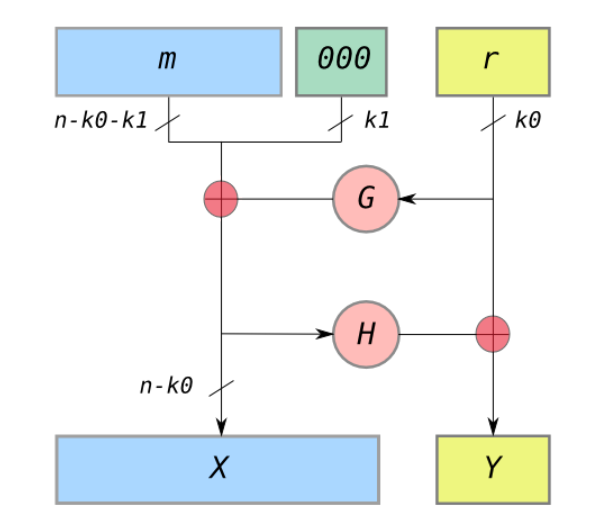
\includegraphics[width=0.8\textwidth]{img/Oaep-diagram-20080305.png}

Al final del procedimiento tenemos:
\[\left\{\begin{array}{l} X = m||0...0 + G(r) \\ Y=r+H(X)\end{array}\right.\]

\end{center}

Con esto podemos ver que los mensajes $m$, por muy pequeños que fuesen, quedarán convertidos en una secuencia aleatoria de caracteres de tamaño $n$.

Una vez tenemos $X||Y$, lo enviamos al destinatario empleando RSA y cifrando $X||Y$ con la clave pública del destino (como hacemos siempre con RSA).

El destinatario puede realizar el descifrado del mensaje como hemos visto siempre y procede a deshacer las operaciones realizadas para recuperar $m$ a partir de $X||Y$.

Para deshacer el \textbf{padding} calcula:
\[\left\{ \begin{array}{l} X \to H(X) \\
r=Y\oplus H(X) \\
m||0...0 = X\oplus G(X)\end{array}\right.\]

\section{Cifrado y firma con RSA}

Como ya hemos visto anteriormente, si tenemos una serie de usuarios que se comunican empleando un criptosistema de clave pública-privada, como puede ser RSA, la forma de garantizar la autenticidad del mensaje consiste en el empleo de las firmas.

Si $A$ quiere enviarle un mensaje a $B$, garantizando que es $A$, lo que enviará será:
\[f_A^{-1}\left(f_B(m)\right) = c\]
puesto que sólo $A$ conoce $f^{-1}_A$.

El usuario $B$, para descifrar el mensaje calculará:
\[m = f_B^{-1}\left(f_A(c)\right)\]

\section{Elección de primos para RSA}

Para empezar, y de manera obvia, los primos $p,q$ tales que $n=p\cdot q$ empleados en el criptosistema deben cumplir unas ciertas propiedades, a fin de evitar que sean descubiertos fácilmente:
\begin{enumerate}
\item Deben ser escogidos al azar
\item No pueden ser pequeños, ni primos de Fermat, ni alguno de los primos más grandes conocidos. En general no pueden ser primos presenten en ningún tipo de tabla, puesto que el atacante también tendrá acceso a esa tabla.
\item No pueden ser de primos cercanos, puesto que la idea de Fermat ayuda a factorizar
\item Tampoco deben ser primos muy lejanos. Deben tener el mismo número de cifras. El método de Polland de curvas elípticas depende del tamaño del menor factor.
\item El mínimo común múltiplo de $p-1$ y $q-1$ debe ser grande puesto que, como se puede ver en el primer ejercicio de la hoja 4, calcular un inverso módulo $a\cdot b$ es equivalente a calcular el inverso en módulo $m.c.m.(a,b)$
\item En resumen hay que evitar cualquier cosa que facilite factorizar $n$ o más exactamente, encontrar el un $d$ que funcione.
\end{enumerate}

\textbf{El procedimiento habitual para conseguir estas propiedades es el siguiente}:
\begin{enumerate}
\item Elijo al azar primos $p',q'$ con los mismos números de dígitos, asegurando que no estarán en ninguna tabla, ni serán demasiado cercanos ni lejanos.

\item Calculo $p=λp'+1$ y $q=μq'+1$ con \textbf{λ,μ pequeños} hasta que $p$ y $q$ sean primos.

Sabemos que este paso funciona por el \textbf{Teorema de Dirichlet} para primos en progresión aritmética, que garantiza que en una progresión aritmética siempre hay infinitos primos, que se equidistribuyen entre todas las progresiones con razones primas menores que $p-1$.

Con esto garantizamos que, puesto que λ y μ son pequeños
\[m.c.d(p-1,q-1) = m.c.d.(λ,μ) \text{ que es pequeño }\]
\end{enumerate}

\section{Otros criptosistemas de clave pública}

A partir de la dificultad de factorizar en primos números grandes surge la idea de RSA.

Otro problema que hemos visto hasta ahora es el del logaritmo discreto, que es aprovechado para idear un criptosistema conocido como \concept{ElGammal}, en honor a su creador, un egipcio que inventó el criptosistema en torno a 1984.

Veamos los pasos a seguir para emplear este sistema:
\begin{enumerate}
\item Tomamos un grupo cíclico $G=<g>$ con $|G| >> 0$

\item Cada usuario elige al azar su exponente $d_i$ secreto y establece como clave pública $e_i=g^{d_i}$.

Conocer el exponente a partir de la clave pública es un problema de logaritmo discreto que sabemos no puede resolverse en tiempo polinómico.

\item Para cifrar tomamos mensajes en $G$, para lo que seleccionamos un primo $p$ tal que:
\[\ent_N \subset \mathbb{F}_p^*\]
siendo $N$ la longitud de los mensajes que cifraremos.
\end{enumerate}

En el momento de enviar un mensaje al usuario $A$, el procedimiento a seguir es:
\begin{enumerate}
\item El usuario $B$ mira $e_A$, elige al azar $1<k<|G|$ y envía:
\[c=(c_1,c_2)=(g^k,me_A^k)\]

\item El usuario $A$ toma $e_A^k = (g^{d_A})^k = (g^k)^{d_A}=c_1^{d_A}$. Puesto que  este usuario es capaz de calcular el opuesto de $d_A$, puede calcular
\[m = c_2\cdot c_1^{-d_A}\]
\end{enumerate}

Para poder atacar a este sistema es necesario conocer $d_A$, que es secreto o $k$ que es secreto y además cambia en cada comunicación.